\documentclass[a4paper]{report}
\usepackage{amsmath}
\usepackage{color}
\usepackage{graphicx}

\begin{document}
\title{Mufasa Handbook}
\author{Merlijn Wajer \and Raymond van Veneti\"{e}}

\maketitle
\tableofcontents

\chapter{Foreword}

This document is aimed at proving a more in depth description on the
functions in the Mufasa Macro Library, and it's extensions.
This can vary from developer notes to extensive explanations on certain
algorithms. \\
Developer notes include:
\begin{itemize}
	\item Implementation Decisions
	\item Bugs
\end{itemize}

\chapter{Core}

\section{TClient}

The TClient class bundles all the other Core classes.
It's main use is to make using the Mufasa Macro Library trivial, by bundling
the core Mufasa classes into one class, and providing the methods to make those
classes cooperate. The main function of this class is to provide a
ready-to-use class that contains all the core functionality of the MML.

\section{MufasaTypes}

MufasaTypes contains all the commonly used types, enums and other constants.
Most of the core classes will use this unit.

\section{TMWindow}

The TMWindow class provides a user with a cross platform API with commonly used
functions like retrieving pixel data of a specified window.

\begin{center}
	\begin{figure}[ht]
		\includegraphics[scale=0.4]{Pics/TMWindow.png}
		\caption{Quick overview of TMWindow}
	\end{figure}
\end{center}

\subsection{Main features}

Retreiving information from the target Application/Window.
\begin{itemize}
	\item Pixel data of a window.
	\item Width and Height of a window.
\end{itemize}

Aside from this core functionality, it also allows programmers to easily switch
between several different targets. It is even allowed to set a memory pointer to
pixel data as target ``window''. It also implements a feature called ``Data
Freeze''.

\subsection{Other important units}

The WindowUtil unit is required for it's X error handler procedure. It also
contains a few other procedures used for XImage to RawImage conversions, but
those aren't used in the TMWindow class.

\subsection{ReturnData}

Return data returns a TRetData structure which contains a pointer to the 
raw image data, and a small description on how to handle the given data.
If it fails, it will return nil on Linux. On Windows, the results may vary.

\subsubsection{TRetData}
\begin{verbatim}
  TRetData = record
    Ptr : PRGB32;
    IncPtrWith : integer;
    RowLen : integer;
  end;
\end{verbatim}

The Ptr contains the data pointer, IncPtrWith contains the value you have to
increase your own data pointer with on a line end, and RowLen contains the
amount of pixels per row. 

\subsection{GetDimensions}

GetDimensions returns the width and height of the currently targetted window.
GetDimensionBox returns the start of the window (left top) and the end of the
window (right bottom).

\subsection{Set Target}

Several SetTarget calls are implemented. Most can be found in the descriptive
picture of TMWindow in the start of this section.
A special call ``SetDesktop'' sets the current window to the
default\footnote{Desktop} window.

\subsection{Freeze}

Freeze is a state that we have implemented in TMWindow. If Freeze is called, the
current client's pixel data is fully copied to an internal bitmap, and
\textbf{all} the next TMWindow calls that are called using the internal data
instead. Once \textbf{Unfreeze} is called, the internal data is freed, and
TMWindow will revert back to it's ``real'' client.

\subsection{Notes on Linux}

On Linux X11 is mainly used for any graphical interface. Any errors generated
by X11 result in a program kill, and X11 will then write the errors. This can be
avoided by setting a custom error handler. This is what we did. Unfortunately we
cannot use the results of the error handler, since we have not been able to
determine a way to make a thread safe error handler. \\
Currently it is mainly in to not make the program brutally crash. You should
however, not encounter any X11 errors.

\section{TMInput}

The \textbf{TMInput} Class is the class that takes care of all the input. \\
MML aims to support both Silent and non Silent Input, although most of the
silent input methods are highly experimental, and need a lot of work.
Since the Input heavily differs per operating system, 
the Input class has a general way of sending keys, possibly at the expense
of losing some Operating System specific functionality. \\

TMInput isn't just used to send keys and mouse presses, but also used to get the
mouse position, or states of keys on the keyboard.

\begin{figure}[ht]
	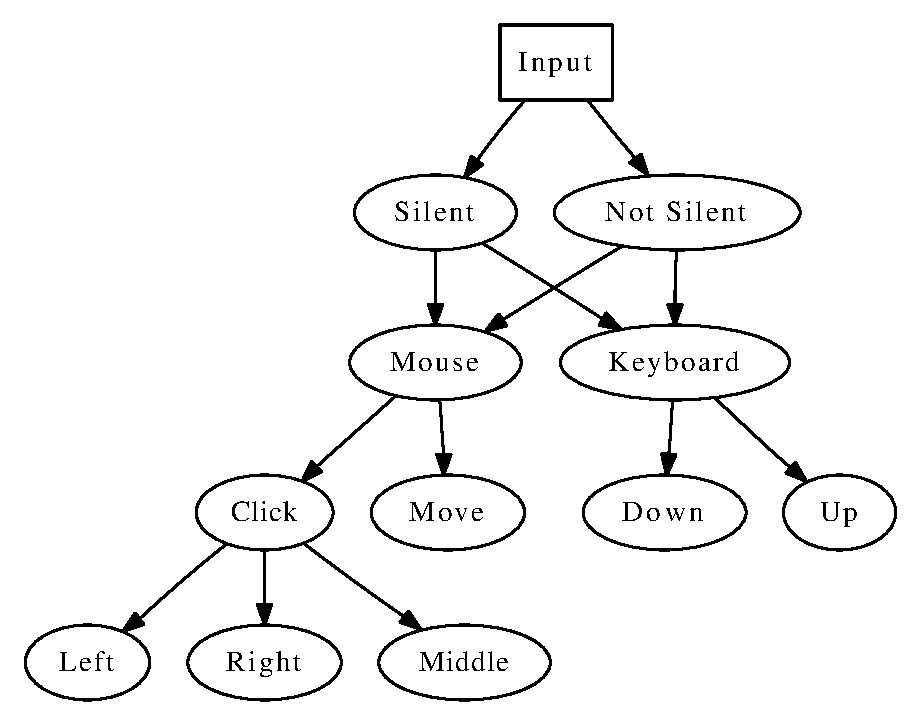
\includegraphics[scale=0.4]{Pics/Input_Diag}
	\caption{Input Functionality.}
\end{figure}

\subsection{Sending Key Input}

% TODO Explain API for keys and mouse.

\subsection{Silent Input}

So what is Silent Input?
We\footnote{Developers of Mufasa} define Silent Input as
methods to manipulate the user's mouse and keyboard, without visually using
them. So what does this mean? \\

This basically means that you will still be able to use your mouse while
MML is performing mouse operations on your targetted window/client.

However, silent input is very hard to implement, and often hardly supported
by host operating systems. Often silent mouse or keyboard input is simply 
ignored. So in general it is advised to stick to non silent input.

\subsubsection{Silent Input On Linux}
It is safe to assume that on Linux, one uses the X.org X11 server for all the
graphical stuff. X11 should allow events to be send to any window, but the
window itself is free to ignore input that may not come from a ``valid'' window.
This makes it harder to implement. However, recently we found a tool called
``xdotool'', which seems to be able to sent silent keys, and possibly mouse
events. Perhaps if we take a better look at it we can work a way out to do
silent input on Linux.

\subsubsection{Silent Input On Windows}
% TODO

\section{TMufasaBitmap}

For the MML, we wrote our own Bitmap class.
A bitmap is basically just a piece of bytes, ordered in a certain fashion.
We have extended this concept to a full blown Bitmap class: ``TMufasaBitmap''.
The data per pixel consists out of 32 bits\footnote{4 bytes}, and is 
``stored'' in the variable ``FData'', of the type ``TRGB32''.
FData is a pointer to the data in memory.
The advantage of a 32 bit structure to a 24 bits structure, consists mainly
of the fact that 32 bits are more easily accessed that 24 bits. 32 bits are
aligned in such a way that they are easily accessed, and translated to
other formats\footnote{Or just ``Colours''}.

\subsection{Converting to and from TMufasaBitmap}

Because there are many other commonly used bitmap classes out there, it is
important that is it easy to ``import'' and ``export'' bitmaps. This may seem
trivial - but there are a lot of things you have to take in account when
importing or exporting. Alignment of bits, the byte order, the line ending
style, the amount of bytes per pixel, etc.

To turn a bitmap into a TMufasaBitmap, we provide two functions.

\begin{verbatim}
    procedure LoadFromTBitmap(bmp: TBitmap);
    procedure LoadFromRawImage(RawImage: TRawImage);
\end{verbatim}

Tbitmap is a commonly used class in Lazarus, and also allows importing and
exporting to many other types. This allows us to load virtually any type that
TBitmap supports. A RawImage is a complex structure of a bitmap ``definition''.
It is commonly used in Lazarus, thus we implemented support for it.

Exporting TMufasaBitmap is done by using the \textbf{ToTBitmap} function. As
mentioned, this allows one to save it to virtually any format.

\subsection{Loading from and Saving to files}

The functions LoadFromFile and SafeToFile allow the programmer to load and safe
TMufasaBitmaps to files. Not all types of bitmap represenations are supported.

%TODO add list of supported bitmaps.

\subsection{Bitmap manipulation}

We also provide some functions that can be used to manipulate bitmaps.
Grayscaling, changing brightness and contrast, posterize and working with
transparent colours are also supported.

\subsection{Copying the Client Window to a TMufasaBitmap}

Coopying the Client Window set in TMWindow is very simply with the TMufasaBitmap
class, just use the \textbf{CopyClientToBitmap} functions.


\section{TMDTM}

The TMDTM class is a DTM manager. It provides methods to add, store, load
and free DTM's. It has a few few other features. One of it's other features
is keeping track of what DTMs are unfreed. It can, for example, help you find
a bug in your code, by printing out information of the DTM that you forgot to
free. You can also give names to DTMs, which eases debugging even further.

If you try to access an invalid DTM, the MML will throw an exception.


\subsection{AddDTM}
\subsection{GetDTM}
\subsection{DTMFromString}
\subsection{FreeDTM}

\section{TMFinder}

\section{TMOCR}
\subsection{Font Loader}
\section{TMFiles}

\chapter{Addon}

\section{Settings Management}

\section{Updater}

\section{Colour Picker}

\section{Window Selector}

\section{Pascal Script Integration}

\section{Plugins}

\end{document}
